\documentclass[11pt,a4paper]{article}
\usepackage[a4paper,hmargin=1in,vmargin=1in]{geometry}
\usepackage{pgfplots}
\pgfplotsset{compat=1.17}

\usepackage[czech]{babel}
\usepackage[utf8]{inputenc}
\usepackage[T1]{fontenc}

\usepackage{stddoc}
\usepackage{lipsum}
\usepackage{subcaption}

\newcommand{\plus}{{\texttt{+}}}
\renewcommand{\Re}{\operatorname{Re}}
\renewcommand{\Im}{\operatorname{Im}}
\newcommand{\fourier}[3]{\mathcal{F}_{#1}\!\left[#2\right]\!\left(#3\right)}
\newcommand{\ifourier}[3]{\mathcal{F}^{-1}_{#1}\!\left[#2\right]\!\left(#3\right)}


\begin{document}

\pagenumbering{arabic}

% Header
\begin{center}
    {\LARGE\textbf{Laboratorní úloha č. 7}}\\[3mm]
    \begin{minipage}{0.4\textwidth}
        \begin{flushleft}
            \textsc{\today}
        \end{flushleft}
    \end{minipage}
    ~
    \begin{minipage}{0.4\textwidth}
        \begin{flushright}
            \textsc{Martin Šimák}
        \end{flushright}
    \end{minipage}
    \noindent\rule{14.5cm}{0.4pt}
\end{center}

\paragraph*{Měření velkosignálových vlastností mikrovlnných směšovačů a násobičů} Laboratorní úloha ukazuje možnosti měření mikrovlnného výkonu termálním a diodovým detektorem a vysílaného pulzního radarového senzoru.

\subsection*{Úkoly měření}
\begin{enumerate}
    \item Měření dodaného výkonu do záteže přes směrovou odbočnici
    \item Měření efektivního vysílaného isotropického výkonu (EIRP) radaru
\end{enumerate}

\subsection*{Použité přístroje a komponenty}
\begin{itemize}
    \item Spektrální analyzátor R\&S FSW26 (2~Hz až 26,5~GHz)
    \item Harmonický mixér R\&S FS-Z90 (60~GHz až 90~GHz)
    \item Trychtýřová anténa RFspin H-A90-W25 (60~GHz až 90~GHz)
    \item Detektor R\&S NRP40TN (DC až 40~GHz)
    \item Detektor Giga-tronics 80401A (0,01~MHz až 18~GHz)
    \item Vyhodnocovací jednotka detektoru Giga-tronics 8541C
    \item Generátor ELSY SG3000 (100~kHz až 3~GHz)
    \item Nízkofrekvenční generátor RIGOL DG2041A (do 40~MHz)
    \item Směrová odbočnice Tesla CGN 102 10 (1~GHz až 2~GHz)
    \item Dělič výkonu Mini-Circuits ZX10-2-20-S\plus\ (200~MHz až 2~GHz)
    \item Integrovaná milimetrová jednotka (IMJ)
    \item Generátor Agilent E8257D (250~kHz až 50~GHz)
    \item Kabely s N konektorem (Pasternack PE302-24)
    \item Propojovací SMA kabely
\end{itemize}

\subsection*{Měřené komponenty}
\begin{itemize}
    \item Radarový modul Texas Instruments AWR1642BOOST (77~GHz až 81~GHz)
\end{itemize}

\subsection*{Popis měření}

% Task 1
\paragraph*{Porovnání možností diodového a termálního detektoru - demonstrace} \lipsum[1]
\begin{figure}[!ht]
    \centering
    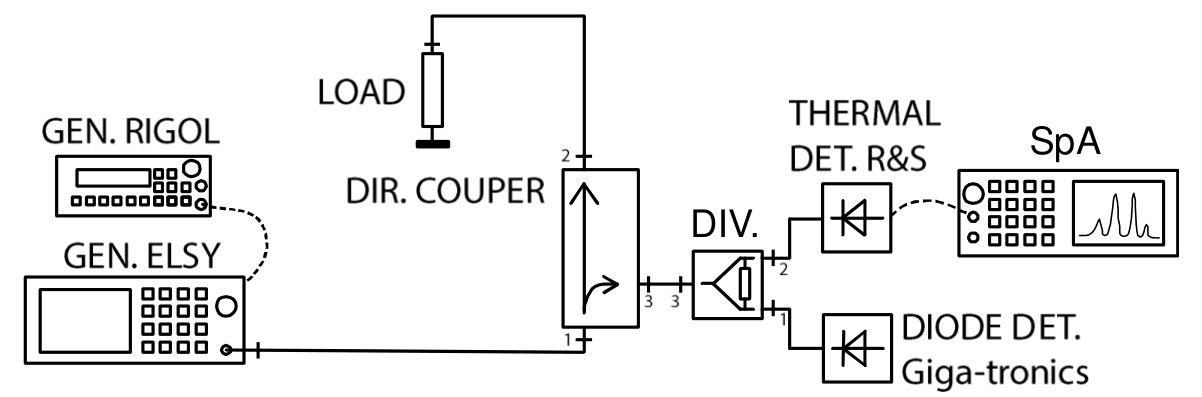
\includegraphics[width=.8\textwidth]{src/task1-zapojeni.png}
    \label{fig:task1-zapojeni}
    \caption{Schéma zapojení úlohy}
\end{figure}

% Task 2
\paragraph*{Měření dodaného výkonu do zátěže přes směrovou odbočnici} Cílem úlohy je ukázat, jak lze měřit výkon dodaný do zátěže nepřímo přes směrovou odbočnici. Ve vysílací technice, kde jsou k anténě dodávány minimálně jednotky wattů výkonu, nelze často měřit výkon přímo, protože běžné mikrovlnné detektory nemají dostatečně velký rozsah měřených výkonů. Zároveň se vysílaný výkon průběžně monitoruje a je součástí smyčky ALC (automatic leveling control). Schéma zapojení úlohy je na obrázku~\ref{fig:task2-zapojeni}.
\begin{figure}[!ht]
    \centering
    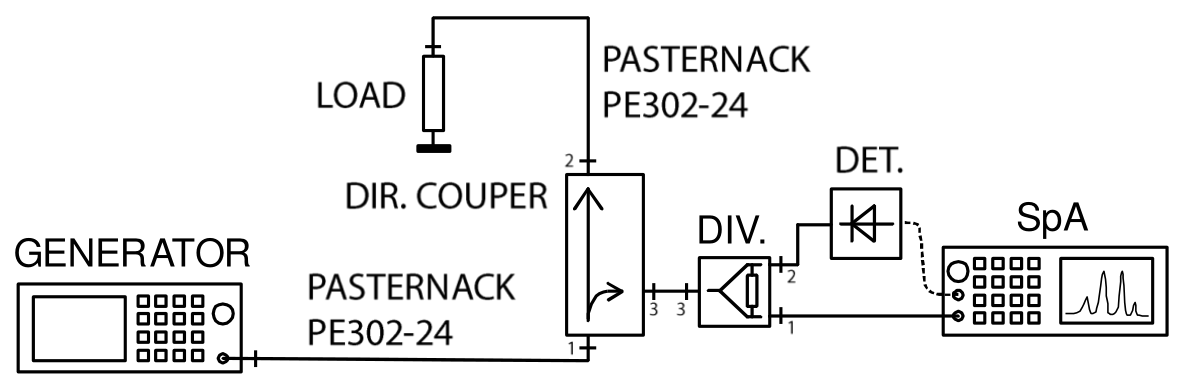
\includegraphics[width=.8\textwidth]{src/task2-zapojeni.png}
    \caption{Schéma zapojení úlohy}
    \label{fig:task2-zapojeni}
\end{figure}

V této úloze slouží spektrální analyzátor jako zobrazovací jednotka pro výkon měřený termálním detektorem a dále detektor informuje o frekvenci vysílaného signálu. Do zátěže se vysílá jen CW signál. Nastavení přístrojů:
\begin{itemize}
    \item vypnutá modulace ASK generátoru,
    \item frekvence výstupního signálu generátoru na 1~GHz a výkon 0~dBm,
    \item spektrální analyzátor s frekvenčním rozsahem měření od 0,9~GHz do 2,1~GHz, jinak v základním nastavení,
    \item svižné měření detektoru s korekcí změřené hodnoty výkonu podle měření frekvence z interních kalibračních dat (\emph{Continuous Update: On}, \emph{Frequency Coupling: Marker}).
\end{itemize}
Po zapnutí detektoru (\emph{Power Sensor Config--State: On}) a nastavení markeru tak, aby vždy sledoval špičku s nejvyšším měřeným výkonem (\emph{Marker Config--Auto Max Peak: On}), na generátoru postupně měníme frekvenci signálu v rozsahu 1~Ghz až 2~GHz, tedy v rozsahu funkčnosti směrové odbočnice, a výkony $P_{\mathrm{DET}}$ změřené detektorem jsou zaznamenány v tabulce~\ref{table:task2-data}.
\begin{table}[!ht]
    \centering
    \begin{tabular}{|l||c|c|c|c|c|c|c|c|c|c|}
        \rule{2cm}{0pt} & \rule{1.5cm}{0pt} & \rule{1.5cm}{0pt} & \rule{1.5cm}{0pt} & \rule{1.5cm}{0pt} & \rule{1.5cm}{0pt}\\[-\arraystretch\normalbaselineskip]
        \hline
        $f\ [\mathrm{MHz}]$ & 1100 & 1200 & 1300 & 1400 & 1500\\
        \hline
        $P_{\mathrm{DET}} \ [\mathrm{dBm}]$ & -17,52 & -17,57 & -17,76 & -17,78 & -17,91\\
        \hline
        $P_{\mathrm{LOAD}} \ [\mathrm{dBm}]$ & -11.7 & -11.7 & -11.9 & -11.9 & -12\\
        \hline\hline
        $f\ [\mathrm{MHz}]$ & 1600 & 1700 & 1800 & 1900 & 2000\\
        \hline
        $P_{\mathrm{DET}} \ [\mathrm{dBm}]$ & -17,87 & -18,14 & -18,31 & -18,35 & -18,80\\
        \hline
        $P_{\mathrm{LOAD}} \ [\mathrm{dBm}]$ & -11.9 & -12.1 & -12.2 & -12.8 & -12.6\\
        \hline
    \end{tabular}
    \caption{Naměřené a vypočítané hodnoty výkonu}
    \label{table:task2-data}
\end{table}

Výkon změřený přes směrovou odbočnici není ten, který je dodáván do zátěže. K dispozici máme
změřené S-parametry dvou stejných kabelů Pasternack, použité směrové odbočnice a děliče vý-
konu. V programu AWR lze tak jednoduše sestavit obvod z bloků S-parametrů jako na obrázku~\ref{fig:task2-sparametry}.
\begin{figure}[!ht]
    \centering
    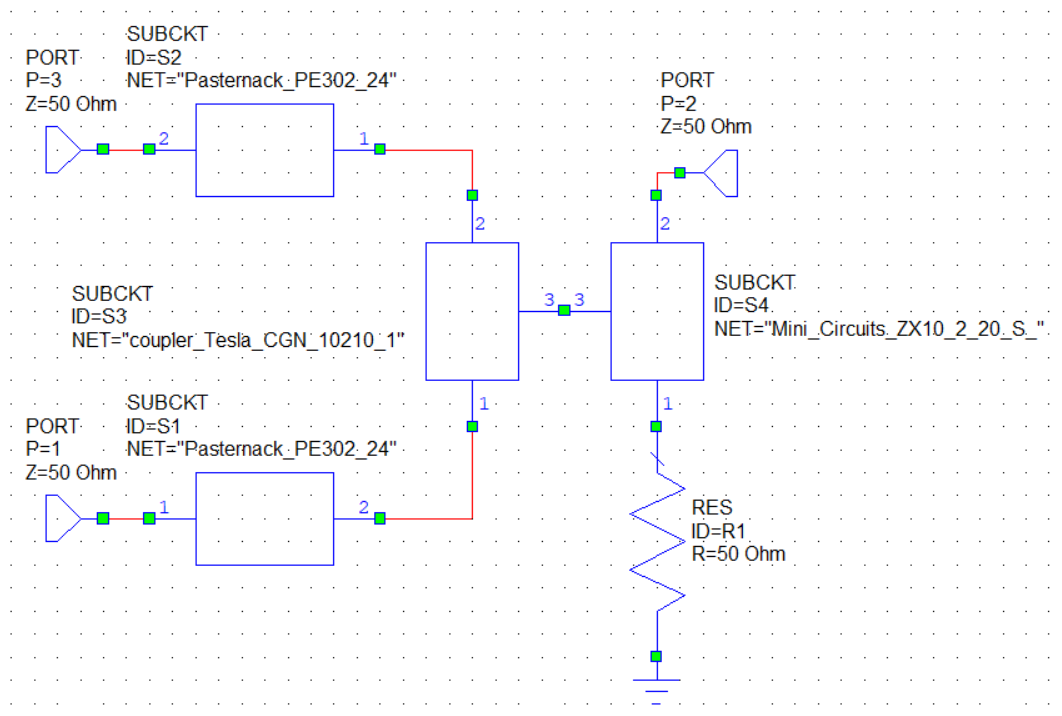
\includegraphics[width=.8\textwidth]{src/task2-sparametry.png}
    \caption{Schéma sestavené z bloků S-parametrů}
    \label{fig:task2-sparametry}
\end{figure}
Měření výkonu $P_{\mathrm{DET}}$ bylo provedeno v místě portu 2 a předpokládáme, že detektor i vstup spektrálního analyzátoru byl bezodrazový. Ze známého výkonu generátoru $P_{\mathrm{in}}$ se dá detekovaný výkon spočítat jako
\begin{align}
    P_{\mathrm{DET}} = P_{\mathrm{in}} \left|S_{21}\right|.
\end{align}
Výkon dodávaný do zátěže se dá pak spočítat jako
\begin{align}
    P_{\mathrm{LOAD}} = P_{\mathrm{in}} \left|S_{31}\right| = P_{\mathrm{DET}} \frac{\left|S_{31}\right|}{\left|S_{21}\right|},
\end{align}
tedy bez potřeby znát skutečnou hodnot výkonu $P_{\mathrm{in}}$ generovaného přímo generátorem. Hodnoty $P_{\mathrm{LOAD}}$ v tabulce~\ref{table:task2-data} jsme získali touto metodou, kde S-parametry byly získány simulací obvodu~\ref{fig:task2-sparametry}. Grafy těchto hodnot jsou znázorněny na obrázku~\ref{fig:task2-sparameter-data}.
\begin{figure}[!ht]
    \centering
    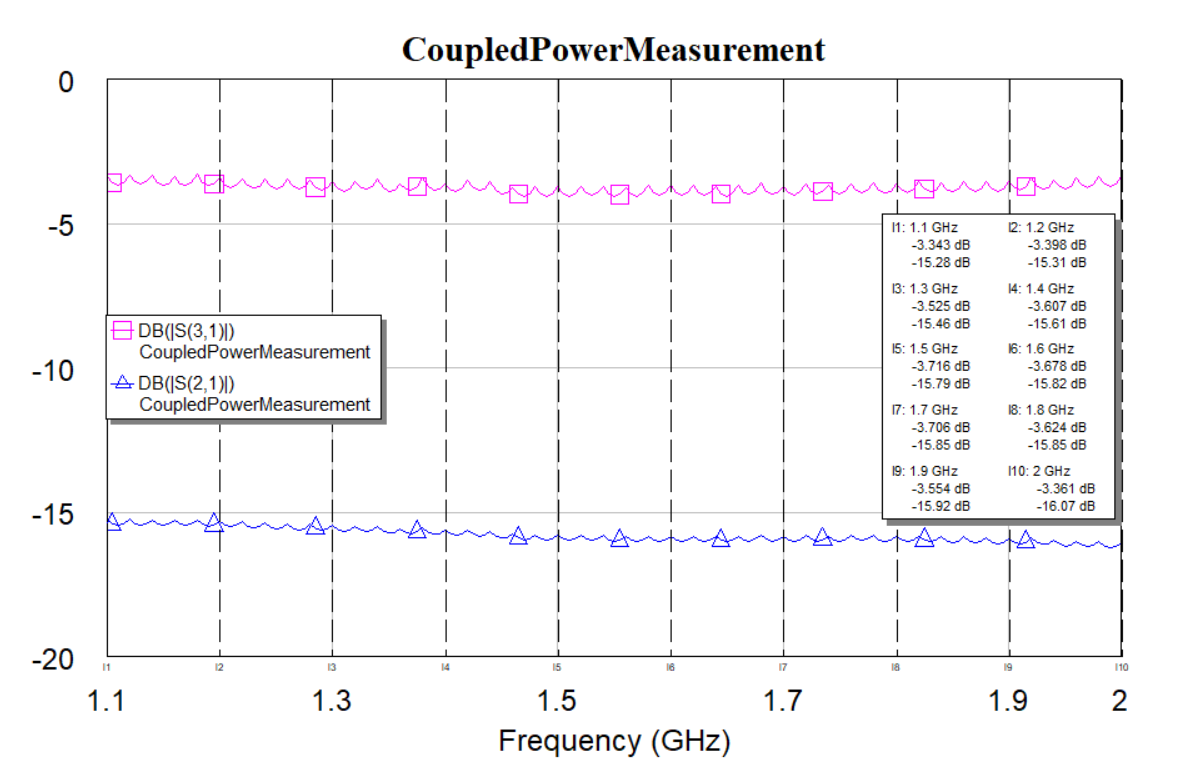
\includegraphics[width=.8\textwidth]{src/task2-sparameter_data.png}
    \caption{S-parametry soustavy odbočující měřený výkon}
    \label{fig:task2-sparameter-data}
\end{figure}

% Task 3
\paragraph*{Měření harmonického signálu pomocí harmonického mixéru - demonstrace} \lipsum[1]
\begin{figure}[!ht]
    \centering
    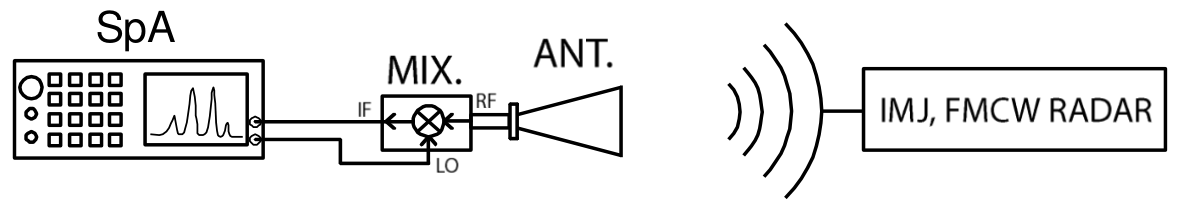
\includegraphics[width=0.8\textwidth]{src/task3-zapojeni.png}
    \caption{Schéma zapojení úlohy}
    \label{fig:task3-zapojeni}
\end{figure}

% Task 4
\paragraph*{Měření EIRP radaru} Zapojení je ponecháno z předchozí úlohy, viz obrázek~\ref{fig:task3-zapojeni}.
\begin{table}[!ht]
    \centering
    \begin{tabular}{|l||c|c|c|c|c|}
        \rule{2cm}{0pt} & \rule{1cm}{0pt} & \rule{1cm}{0pt} & \rule{1cm}{0pt} & \rule{1cm}{0pt} & \rule{1cm}{0pt}\\[-\arraystretch\normalbaselineskip]
        \hline
        $f \ [\mathrm{GHz}]$ & 77 & 78 & 79 & 80 & 81\\
        \hline
        $P_{\mathrm{RX}} \ [\mathrm{dBm}]$ & X & X & X & X & X\\
        \hline
        $\mathrm{FSL} \ [\mathrm{dB}]$ & X & X & X & X & X\\
        \hline\hline
        $\mathrm{EIRP} \ [\mathrm{dBm}]$ & X & X & X & X & X\\
        \hline
    \end{tabular}
    \caption{Naměřená a vypočítaná data}
    \label{table:task4-data}
\end{table}

% Task 5
\paragraph*{Měření rychlých dějů pomocí real-time spektra - demonstrace} \lipsum[1]


\subsection*{Závěr}
\lipsum[1]


\end{document}
